Ein Weg, der in einem unbegrenzten Dreiecksgitter
von einem Punkt jeweils zu einem der sechs Nachbarpunkte führt,
kann als Folge von Segmenten mit den Richtungen \texttt{a} bis \texttt{f}
beschrieben werden:
\begin{center}
\begin{tikzpicture}[>=latex,thick]
\coordinate (A) at (0.5,{sqrt(3)/2});
\coordinate (E) at (1,0);
\coordinate (O) at (0,0);
\def\punkt#1#2{
	\fill[color=white] ($#1*(E)+#2*(A)$) circle[radius=0.10];
	\fill[color=gray] ($#1*(E)+#2*(A)$) circle[radius=0.06];
}
\draw[line width=0.2pt,color=gray] ($-3*(E)-0.5*(A)$) -- ($-3*(E)+3.5*(A)$);
\draw[line width=0.2pt,color=gray] ($-2*(E)-1.5*(A)$) -- ($-2*(E)+3.5*(A)$);
\draw[line width=0.2pt,color=gray] ($-1*(E)-2.5*(A)$) -- ($-1*(E)+3.5*(A)$);
\draw[line width=0.2pt,color=gray] ($-0*(E)-3.5*(A)$) -- ($-0*(E)+3.5*(A)$);
\draw[line width=0.2pt,color=gray] ($+1*(E)-3.5*(A)$) -- ($+1*(E)+2.5*(A)$);
\draw[line width=0.2pt,color=gray] ($+2*(E)-3.5*(A)$) -- ($+2*(E)+1.5*(A)$);
\draw[line width=0.2pt,color=gray] ($+3*(E)-3.5*(A)$) -- ($+3*(E)+0.5*(A)$);

\draw[line width=0.2pt,color=gray] ($-3.5*(E)+3*(A)$) -- ($+0.5*(E)+3*(A)$);
\draw[line width=0.2pt,color=gray] ($-3.5*(E)+2*(A)$) -- ($+1.5*(E)+2*(A)$);
\draw[line width=0.2pt,color=gray] ($-3.5*(E)+1*(A)$) -- ($+2.5*(E)+1*(A)$);
\draw[line width=0.2pt,color=gray] ($-3.5*(E)+0*(A)$) -- ($+3.5*(E)+0*(A)$);
\draw[line width=0.2pt,color=gray] ($-2.5*(E)-1*(A)$) -- ($+3.5*(E)-1*(A)$);
\draw[line width=0.2pt,color=gray] ($-1.5*(E)-2*(A)$) -- ($+3.5*(E)-2*(A)$);
\draw[line width=0.2pt,color=gray] ($-0.5*(E)-3*(A)$) -- ($+3.5*(E)-3*(A)$);

\draw[line width=0.2pt,color=gray] ($-3.5*(E)+0.5*(A)$) -- ($+0.5*(E)-3.5*(A)$);
\draw[line width=0.2pt,color=gray] ($-3.5*(E)+1.5*(A)$) -- ($+1.5*(E)-3.5*(A)$);
\draw[line width=0.2pt,color=gray] ($-3.5*(E)+2.5*(A)$) -- ($+2.5*(E)-3.5*(A)$);
\draw[line width=0.2pt,color=gray] ($-3.5*(E)+3.5*(A)$) -- ($+3.5*(E)-3.5*(A)$);
\draw[line width=0.2pt,color=gray] ($-2.5*(E)+3.5*(A)$) -- ($+3.5*(E)-2.5*(A)$);
\draw[line width=0.2pt,color=gray] ($-1.5*(E)+3.5*(A)$) -- ($+3.5*(E)-1.5*(A)$);
\draw[line width=0.2pt,color=gray] ($-0.5*(E)+3.5*(A)$) -- ($+3.5*(E)-0.5*(A)$);

\foreach \x in {-3,...,0}{ \punkt{\x}{+3} }
\foreach \x in {-3,...,1}{ \punkt{\x}{+2} }
\foreach \x in {-3,...,2}{ \punkt{\x}{+1} }
\foreach \x in {-3,...,3}{ \punkt{\x}{0} }
\foreach \x in {-2,...,3}{ \punkt{\x}{-1} }
\foreach \x in {-1,...,3}{ \punkt{\x}{-2} }
\foreach \x in {-0,...,3}{ \punkt{\x}{-3} }

\draw 	   ($-2*(E)-2*(A)$)
	-- ($+1*(E)-2*(A)$)
	-- ($+1*(E)-1*(A)$)
	-- ($+2*(E)-1*(A)$)
	-- ($+2*(E)+2*(A)$)
	-- ($-2*(E)+2*(A)$)
	-- cycle;

\definecolor{farbeeins}{rgb}{0.8,0.4,0.8}
\definecolor{farbezwei}{rgb}{0.8,0.4,0.4}
\definecolor{farbedrei}{rgb}{0.8,0.8,0.4}
\definecolor{farbevier}{rgb}{0.4,0.8,0.4}
\definecolor{farbefuenf}{rgb}{0.4,0.8,0.8}
\definecolor{farbesechs}{rgb}{0.4,0.4,0.8}

\draw[->,color=farbeeins] (O) -- (E);
\node[color=farbeeins] at (E) [above left] {\texttt{a}};

\draw[->,color=farbezwei] (O) -- (A);
\node[color=farbezwei] at (A) [left] {\texttt{b}};

\draw[->,color=farbedrei] (O) -- ($-1*(E)+(A)$);
\node[color=farbedrei] at ($-1*(E)+(A)$) [below left] {\texttt{c}};

\draw[->,color=farbevier] (O) -- ($-1*(E)$);
\node[color=farbevier] at ($-1*(E)$) [below right] {\texttt{d}};

\draw[->,color=farbefuenf] (O) -- ($-1*(A)$);
\node[color=farbefuenf] at ($-1*(A)$) [right] {\texttt{e}};

\draw[->,color=farbesechs] (O) -- ($(E)-1*(A)$);
\node[color=farbesechs] at ($(E)-1*(A)$) [above right] {\texttt{f}};

\fill ($-2*(E)-2*(A)$) circle[radius=0.06];

\end{tikzpicture}
\end{center}
Die Wörter der Sprache
\[
L
=
\{
w\in \Sigma^*
\;|\;
\text{$w$ führt zurück zum Startpunkt}
\}
\]
beschreiben geschlossene Pfade. 
Kann man eine kontextfreie Grammatik für $L$ angeben?

\begin{hinweis}
Betrachten Sie Pfade, die nur die Richtungen
\texttt{a},
\texttt{b},
\texttt{d}
und
\texttt{e}
verwenden, wie der eingezeichnete Pfad, der zum Wort
\texttt{aaababbbddddeeee} mit dem Startpunkt in der
linken unteren Ecke gehört.
\end{hinweis}

\begin{loesung}
\definecolor{darkgreen}{rgb}{0,0.8,0}
Geschlossene Pfade der Teilsprache aus den Zeichen
$\Sigma'=\{ \texttt{a}, \texttt{b}, \texttt{d}, \texttt{e} \}$
haben jeweils gleich viele \texttt{a} wie \texttt{d} 
und gleichviele \texttt{b} wie \texttt{e}, werden also durch
Wörter der Sprache
\begin{equation}
L'
=
\{
\Sigma^{\prime *}
\;|\;
|w|_{\texttt{a}}
=
|w|_{\texttt{d}}
\wedge
|w|_{\texttt{b}}
=
|w|_{\texttt{e}}
\}.
\end{equation}
Wäre $L$ kontextfrei, müssten auch die Pfade in $L'$ durch eine Grammatik
beschrieben werden können.
Dies ist aber nicht möglich, weil $L'$ nicht kontextfrei ist, wie man
mit dem Pumping Lemma zeigen kann.
\begin{enumerate}
\item
Wir nehmen an, dass $L'$ kontextfrei ist.
\item
Nach dem Pumping Lemma für kontextfreie Sprachen gibt es die
Pumping Length $N$
\item
Wir nehmen das Wort
$w= \texttt{a}^N \texttt{b}^N \texttt{e}^N \texttt{d}^N $,
es beschreibt einen im Gegenuhrzeigersinn durchlaufenen Rhombus
mit Seitenlänge $N$.
\item
Nach dem Pumping-Lemma gibt es eine Aufteilung des Wortes in
fünf Teile
$w=
{\color{blue}u}
{\color{red}v}
{\color{darkgreen}x}
{\color{red}y}
{\color{blue}z}$
\begin{center}
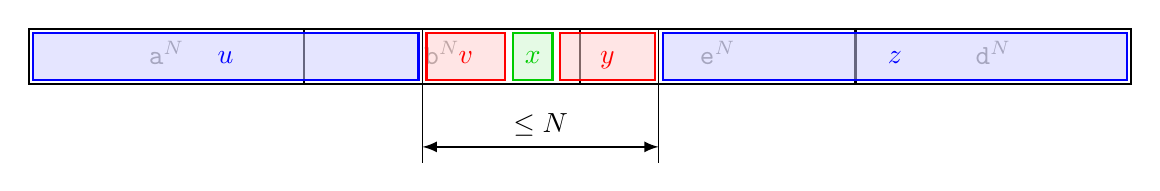
\begin{tikzpicture}[>=latex,thick]
\def\xa{0}
\def\xb{3.5}
\def\xc{7}
\def\xd{10.5}
\def\xe{14}
\def\y{0.7}
\draw (0,0) rectangle (\xe,\y);
\draw (\xb,0) -- (\xb,\y);
\draw (\xc,0) -- (\xc,\y);
\draw (\xd,0) -- (\xd,\y);
\node[color=gray] at ({0.5*(\xa+\xb)},{0.5*\y}) {$\texttt{a}\mathstrut^N$};
\node[color=gray] at ({0.5*(\xb+\xc)},{0.5*\y}) {$\texttt{b}\mathstrut^N$};
\node[color=gray] at ({0.5*(\xc+\xd)},{0.5*\y}) {$\texttt{e}\mathstrut^N$};
\node[color=gray] at ({0.5*(\xd+\xe)},{0.5*\y}) {$\texttt{d}\mathstrut^N$};
\def\s{0.05}
\def\Xb{5}
\pgfmathparse{\Xb+1.1}
\xdef\Xc{\pgfmathresult}
\pgfmathparse{\Xc+0.6}
\xdef\Xd{\pgfmathresult}
\pgfmathparse{\Xd+1.3}
\xdef\Xe{\pgfmathresult}


\def\rechteck#1#2#3#4{
	\fill[color=#3!20,opacity=0.5]
		({#1+\s},\s) rectangle ({#2-\s},{\y-\s});
	\draw[color=#3] ({#1+\s},\s) rectangle ({#2-\s},{\y-\s});
	\node[color=#3] at ({0.5*(#1+#2)},{0.5*\y}) {$#4\mathstrut$};
}

\rechteck{\xa}{\Xb}{blue}{u}
\rechteck{\Xb}{\Xc}{red}{v}
\rechteck{\Xc}{\Xd}{darkgreen}{x}
\rechteck{\Xd}{\Xe}{red}{y}
\rechteck{\Xe}{\xe}{blue}{z}

\draw[line width=0.3pt] (\Xb,\y) -- (\Xb,-1);
\draw[line width=0.3pt] (\Xe,\y) -- (\Xe,-1);
\draw[<->] (\Xb,-0.8) -- (\Xe,-0.8);
\node at ({0.5*(\Xb+\Xe)},-0.8) [above] {$\le N$};

\end{tikzpicture}
\end{center}
mit $|x|>0$ und $|vxy|\le N$ derart,
dass auch die aufgepumpten Wörter $uv^kxy^kz\in L'$ sind.
\item
Wegen $|vxy|\le N$ kann sich beim Pumpen höchstens die Anzahl von
zwei der Buchstaben ändern, niemals aber die Anzahl beider Buchstaben
gleichzeitig, die jeweils gleich sein sollte.
\item
Dieser Widerspruch zeigt, dass $L'$ nicht kontextfrei sein kann
und damit auch $L$ nicht.
\qedhere

\end{enumerate}
\end{loesung}

\begin{bewertung}
Annahme $L$ regulär ({\bf PL}) 1 Punkt,
Pumping Length ({\bf N}) 1 Punkt,
geeignetes Wort wählen ({\bf W}) 1 Punkt,
Unterteilung des Wortes ({\bf U}) 1 Punkt,
Widerspruch beim Pumpen ({\bf P}) 1 Punkt,
Schlussfolgerung ({\bf S}) 1 Punkt.
\end{bewertung}
